%versi 2 (8-10-2016)
\chapter{Landasan Teori}
\label{chap:teori}

\section{Pengujian Perangkat Lunak}
\label{softwaretesting}
\paragraph{}
Pandangan umum pengujian perangkat lunak adalah bahwa kegiatan ini adalah untuk menemukan \textit{bug}. Tujuan pengujian perangkat lunak adalah untuk memenuhi syarat kualitas program perangkat lunak dengan mengukur atribut dan kemampuannya terhadap ekspektasi dan standar yang berlaku. Pengujian perangkat lunak juga menyediakan informasi berharga untuk upaya pengembangan perangkat lunak.[9]

Kualitas perangkat lunak adalah sesuatu yang diinginkan semua orang. Manajer tahu bahwa mereka menginginkan kualitas tinggi, pengembangan perangkat lunak tahu mereka ingin menghasilkan produk yang berkualitas, dan pengguna bersikeras bahwa perangkat lunak bekerja secara konsisten dan dapat diandalkan.[9]

Banyak kelompok kualitas perangkat lunak mengembangkan \textit{software quality assurance plan}, dimana hal itu sama dengan \textit{test plans}. Rencana jaminan kualitas perangkat lunak dapat mencakup berbagai kegiatan di luar yang termasuk dalam \textit{test plan}. \textit{Quality assurance plan} mencakup keseluruhan kualitas, rencana pengujian adalah salah satu alat kontrol kualitas dari rencana jaminan kualitas.[9]

Pada pembahasan pengujian perangkat lunak, ada \textit{term} yang biasa digunakan, yaitu[8]:
\begin{itemize}
\item \textbf{Error} --- Orang membuat \textit{error}. Sinonim yang baik adalah \textit{mistake}. Ketika orang membuat \textit{error} saat melakukan \textit{coding}, kami menyebut \textit{error} ini \textit{bug}. \textit{Error} cenderung menyebar; \textit{requirements error} dapat diperbesar selama proses desain dan lebih diperkuat lagi selama pengkodean.
\item \textbf{Fault} --- \textit{Fault} adalah hasil dari \textit{error}. Lebih tepat untuk mengatakan bahwa \textit{fault} adalah representasi dari \textit{error}, di mana representasi adalah mode ekspresi, seperti teks naratif, diagram Bahasa Pemodelan Bersatu, diagram hierarki, dan kode sumber. \textit{Defect} adalah sinonim yang baik untuk \textit{fault}, sama juga seperti \textit{bug}. \textit{Fault} bisa sulit dipahami. \textit{Error} yang disebakan oleh kelalaian menghasilkan \textit{fault} di mana ada sesuatu yang hilang yang seharusnya ada di dalam representasi.
\item \textit{\textbf{Failure}} --- \textit{Failure} terjadi ketika kode yang sesuai dengan \textit{fault} dijalankan. Dua kehalusan muncul di sini: satu adalah bahwa \textit{failure} hanya terjadi dalam representasi yang dapat dieksekusi, yang biasanya dianggap sebagai kode sumber, atau lebih tepatnya, kode objek yang dimuat; kehalusan kedua adalah bahwa definisi ini hanya mengaitkan \textit{failure} dengan \textit{fault} komisi.
\item \textbf{Incident} --- Ketika \textit{failure} terjadi, itu mungkin atau mungkin tidak mudah terlihat oleh pengguna (atau pelanggan atau penguji). Suatu \textit{incident} adalah gejala yang terkait dengan \textit{failure} yang memberi tahu pengguna tentang terjadinya \textit{failure}.
\item \textbf{Test} --- \textit{Testing} jelas berkaitan dengan  \textit{errors, faults, failures, and incidents}. \textit{Test} adalah tindakan melatih perangkat lunak dengan \textit{test case}. \textit{Test} memiliki dua tujuan berbeda: untuk menemukan \textit{failures} atau untuk menunjukkan eksekusi yang benar.
\item \textbf{Test case} --- \textit{Test case} memiliki identitas dan dikaitkan dengan perilaku program. Ini juga memiliki serangkaian input dan output yang diharapkan.
\end{itemize}
\begin{figure}
	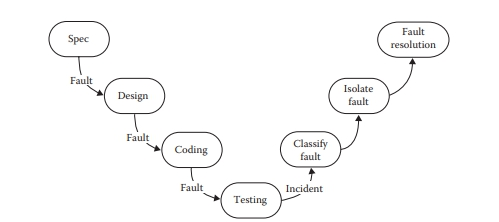
\includegraphics[scale=1.2]{gambar/cycle}
	\centering
	\caption{Siklus hidup pengujian.}
\end{figure}
Gambar 2.1 menggambarkan model siklus hidup untuk pengujian. Perhatikan bahwa, dalam fase pengembangan, tiga peluang muncul untuk membuat \textit{error}, yang menghasilkan \textit{fault} yang dapat menyebar melalui proses \textit{development}. Langkah resolusi \textit{fault} adalah kesempatan lain untuk \textit{error} (dan \textit{fault} baru). Ketika suatu perbaikan menyebabkan perangkat lunak yang sebelumnya benar untuk berperilaku salah, perbaikannya kurang[8].

Dari urutan \textit{term} ini, dapat dilihat bahwa \textit{test case} menempati posisi sentral dalam pengujian. Proses pengujian dapat dibagi lagi menjadi langkah-langkah terpisah: \textit{test planning, test case development}, menjalankan \textit{test case}, dan mengevaluasi hasil pengujian.Untuk \textit{test case} ada dua pendekatan mendasar digunakan untuk mengidentifikasi \textit{test case}; secara tradisional, ini disebut pengujian fungsional dan struktural. \textit{Specification-based} dan \textit{code-based} adalah nama yang lebih deskriptif. Kedua pendekatan memiliki beberapa metode identifikasi \textit{test case} yang berbeda; mereka umumnya hanya disebut metode pengujian.

\subsection{\textit{Specification-Based/Black-box Testing} [8]}
\paragraph{} 
Alasan bahwa pengujian berbasis spesifikasi pada awalnya disebut \textit{functional testing} adalah bahwa setiap program dapat dianggap sebagai fungsi yang memetakan nilai dari domain input ke nilai dalam rentang outputnya. Gagasan ini umumnya digunakan dalam \textit{engineering}, ketika suatu sistem dianggap sebagai \textit{black box}. Ini mengarah pada istilah sinonim lainnya — pengujian \textit{black-box}, di mana konten (implementasi) kotak hitam tidak diketahui, dan fungsi kotak hitam dipahami sepenuhnya dalam hal input dan outputnya (lihat Gambar 2.2). Sering kali, pengujian beroperasi sangat efektif dengan pengetahuan \textit{black box}; pada kenyataannya, ini adalah pusat orientasi objek. Sebagai contoh, kebanyakan orang berhasil mengoperasikan mobil dengan hanya pengetahuan "\textit{black box}".
\begin{figure}[h!]
	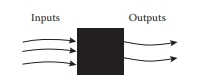
\includegraphics[scale=1.0]{gambar/blackbox}
	\centering
	\caption{Engineer’s black box.}
\end{figure}

Dengan pendekatan berbasis spesifikasi untuk menguji identifikasi kasus, satu-satunya informasi yang digunakan adalah spesifikasi perangkat lunak. Oleh karena itu, \textit{test case} memiliki dua keunggulan berbeda: 
\begin{enumerate}
\item Mereka tidak tergantung pada bagaimana perangkat lunak diimplementasikan, jadi jika implementasi berubah, \textit{test case} masih berguna.
\item Pengembangan \textit{test case} dapat terjadi secara paralel dengan implementasi, sehingga mengurangi keseluruhan interval pengembangan proyek.
\end{enumerate} 
Di sisi negatif, kasus uji berbasis spesifikasi sering mengalami dua masalah, redudansi yang signifikan mungkin ada di antara kasus uji, dan diperparah oleh kemungkinan kesenjangan perangkat lunak yang tidak diuji.

Gambar 2.3 menunjukkan hasil \textit{test case} yang diidentifikasi oleh dua metode berbasis spesifikasi. Metode A mengidentifikasi serangkaian kasus uji yang lebih besar daripada metode B. Perhatikan bahwa, untuk kedua metode, rangkaian kasus uji sepenuhnya terkandung dalam rangkaian perilaku tertentu. Karena metode berbasis spesifikasi didasarkan pada perilaku yang ditentukan, sulit untuk membayangkan metode ini mengidentifikasi perilaku yang tidak ditentukan.
\begin{figure}
	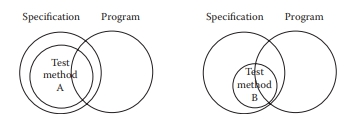
\includegraphics[scale=1.2]{gambar/compareAB}
	\centering
	\caption{Comparing specification-based test case identification methods}
\end{figure}
\subsection{\textit{Code-Based/White-box Testing}[8]}
\paragraph{}
Pengujian berbasis kode adalah pendekatan mendasar lainnya untuk menguji \textit{test case}. Untuk membandingkannya dengan pengujian \textit{black box}, kadang-kadang disebut pengujian \textit{white box} (atau bahkan \textit{clear box}). Metafora \textit{clear box} mungkin lebih tepat karena perbedaan mendasar adalah bahwa implementasi (\textit{black box}) diketahui dan digunakan untuk mengidentifikasi \textit{test case}. Kemampuan untuk "melihat ke dalam" \textit{black box} memungkinkan tester untuk mengidentifikasi \textit{test case} berdasarkan bagaimana fungsi tersebut benar-benar dijalankan.

Pengujian berbasis kode telah menjadi subjek dari beberapa teori yang cukup kuat. Dengan konsep-konsep ini, tester dapat dengan ketat menggambarkan dengan tepat apa yang akan diuji. Karena dasar teorinya yang kuat, pengujian berbasis kode cocok untuk menjadi definisi dan penggunaan \textit{test coverage metrics}. \textit{Test coverage metrics} menyediakan cara untuk secara eksplisit menyatakan sejauh mana \textit{item} perangkat lunak telah diuji, dan ini pada gilirannya membuat manajemen pengujian lebih jelas.
\begin{figure}[h!]
 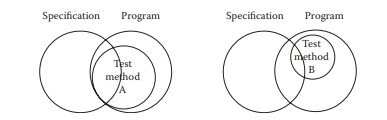
\includegraphics[scale=1.2]{gambar/compareAB-whitebox}
 \centering
 \caption{Comparing code-based test case identification methods.}
\end{figure}
Gambar 2.4 menunjukkan hasil \textit{test case} yang diidentifikasi oleh dua metode berbasis kode. Seperti sebelumnya, metode A mengidentifikasi satu set kasus uji yang lebih besar daripada metode B. Apakah satu set kasus uji yang lebih besar tentu lebih baik? Ini adalah pertanyaan yang bagus, dan pengujian berbasis kode menyediakan cara-cara penting untuk mengembangkan jawaban. Perhatikan bahwa, untuk kedua metode, himpunan kasus uji sepenuhnya terkandung dalam himpunan perilaku yang diprogram. Karena metode berbasis kode didasarkan pada program, sulit membayangkan metode ini mengidentifikasi perilaku yang tidak diprogram. Sangat mudah untuk membayangkan, bagaimanapun, bahwa serangkaian kasus uji berbasis kode relatif kecil sehubungan dengan perilaku lengkap yang diprogram. 

\section{\textit{Unit Testing}[10]}
\paragraph{}
Tahap paling dalam pada pengujian perangkat lunak adalah \textit{unit testing}.Dalam \textit{unit testing}, kita menguji setiap unit kode secara individu, biasanya sebuah \textit{method}, dalam isolasi untuk melihat apakah jika diberikan suatu kondisi tertentu, apakah respons yang didapat akan sama dengan yang diharapkan (lihat Gambar 2.5). Memecah pengujian ke tingkat dasar memberi keyakinan bahwa setiap bagian dari aplikasi akan berperilaku seperti yang diharapkan dan memungkinkan untuk menutupi kasus di mana hal yang tidak terduga dapat terjadi dan menanganinya dengan cara yang tepat.
\begin{figure}[h!]
	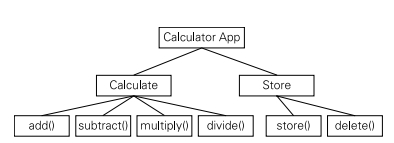
\includegraphics[scale=1.5]{gambar/unittest}
	\centering
	\caption{Contoh struktur aplikasi yang menunjukkan kelas dan method. Method adalah "unit" yang akan diuji.}
\end{figure}

Pada contoh diatas, \textit{method} yang disorot adalah unit individual dari aplikasi ini yang perlu diuji. Jika tahu bahwa masing-masing \textit{method} pada kelas \textit{Calculator} berfungsi seperti yang diharapkan, maka kita yakin bahwa fitur-fitur aplikasi \textit{Calculator} tersebut telah berjalan sesuai harapan.

Misalnya, kita ingin menguji apakah hasil dari \textit{method} dengan dua angka benar-benar menambahkannya untuk menghasilkan jumlah yang benar. Memecah kode menjadi \textit{unit-unit} ini membuat proses pengujian lebih mudah. Saat berurusan dengan \textit{unit} kecil dari sebuah aplikasi, kita memiliki pemahaman yang jelas tentang cara kerja unit tersebut dan hal-hal yang memungkinkan untuk salah pada potongan kode tertentu, sehingga memungkinkan untuk menutupi \textit{unit} dengan tes yang sesuai.

Selain itu, saat melakukan pengujian dengan cara ini biasanya jelas jika kita telah memecah kode menjadi unit-unit. Jika harus menulis banyak tes berbeda untuk mencakup semua kemungkinan berbeda yang dapat dilalui \textit{method} ini, \textit{method} tersebut mungkin terlalu besar dan harus dipertimbangkan untuk melakukan \textit{refactoring} menjadi dua metode atau lebih dengan tanggung jawab yang sama. Sebaliknya, mungkin ada kasus di mana \textit{method} terlalu sederhana dan dapat dikombinasikan dengan beberapa fungsi lain untuk membuat \textit{method} yang lebih berguna. Sebagai seorang \textit{programmer} yang berpengalaman, kita harus mulai merasakan metode mana yang yang sudah "berukuran" baik dan mana yang tidak. Sepuluh baris sering merupakan aturan praktis yang baik untuk diikuti. Sebagai programmer yang baik, kita harus berusaha untuk memberikan kode yang paling mudah dibaca.

Tes yang ditulis adalah cerita yang menjelaskan kode dari sebuah program. Apa yang ingin dibaca atau dilihat ketika pertama kali membaca kode dan mencoba memahami apa fungsinya? Konvensi penamaan variabel yang jelas, ringkas, nama kelas, nama file, dan tes dapat membantu membuat kode lebih jelas dan mudah dipelihara untuk orang lain.

\section{\textit{Behavior-Driven Development}[11]}
Behavior-Driven Development (BDD) adalah seperangkat praktik rekayasa perangkat lunak yang dirancang untuk membantu tim membangun dan memberikan perangkat lunak yang lebih bernilai dan berkualitas lebih cepat. Ini mengacu pada \textit{agile} dan \textit{lean practices} termasuk, khususnya, \textit{Test-Driven Development} (TDD) dan \textit{Domain-Driven Design} (DDD). Tetapi yang paling penting, BDD menyediakan bahasa umum berdasarkan kalimat-kalimat sederhana dan terstruktur yang diekspresikan dalam bahasa Inggris (atau dalam bahasa asli para pemangku kepentingan) yang memfasilitasi komunikasi antara anggota tim proyek dan pemangku kepentingan bisnis.

Untuk lebih memahami cara kerja BDD, dengan BDD yang berevolusi dari TDD, kita harus membahasa sedikit tentang TDD. Test-Driven Development (TDD) adalah praktik pengembangan yang menggunakan \textit{unit test} untuk menentukan, merancang, dan memverifikasi kode yang akan ditulis. Sebelum menerapkan fungsionalitas, \textit{developer} menulis \textit{unit test} yang sengaja digagalkan untuk menunjukkan bagaimana fungsi ini seharusnya bekerja. Pada saat yang sama, pengujian gagal ini juga membuktikan bahwa implementasi saat ini belum mendukung fungsionalitas yang baru. Baru setelah itu \textit{developer} menulis kode program. Setelah \textit{unit testing} berlalu, \textit{developer} tahu bahwa fungsionalitas telah berhasil diimplementasikan. Pada tahap ini, mereka dapat meninjau kode mereka untuk merapikan dan menyempurnakan desain.

BDD pada awalnya dirancang sebagai versi perbaikan TDD. BDD awalnya ditemukan oleh Dan North pada awal hingga pertengahan 2000-an sebagai cara yang lebih mudah untuk mengajar dan mempraktikkan Test-Driven Development (TDD). TDD, ditemukan oleh Kent Beck pada awal munculnya \textit{Agile Development}, itu adalah teknik efektif yang menggunakan \textit{unit test} untuk menentukan, merancang, dan memverifikasi kode program.

Ketika pengguna TDD perlu mengimplementasikan fitur, mereka terlebih dahulu menulis tes gagal yang menjelaskan, atau menentukan fitur itu. Selanjutnya, mereka menulis kode yang cukup untuk lulus melakukan tes kode. Akhirnya, mereka memperbaiki kode untuk membantu memastikan bahwa kode itu akan mudah dirawat (lihat gambar 2.6). Teknik sederhana namun kuat ini mendorong pengembang untuk menulis kode yang lebih bersih, dirancang lebih baik, lebih mudah dirawat dan menghasilkan jumlah kecacatan kode yang jauh lebih rendah.

\begin{figure}
	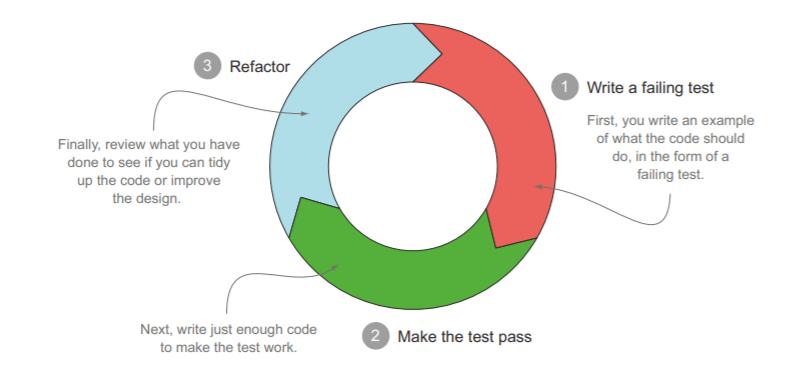
\includegraphics[scale=1.2]{gambar/bdd}
	\centering
	\caption{Test-Driven Development three-phase cycle}
\end{figure}
Terlepas dari kelebihannya, banyak orang masih kesulitan mengadopsi dan menggunakan TDD secara efektif. \textit{Developer} sering mengalami kesulitan mengetahui di mana harus memulai atau tes apa yang harus mereka tulis selanjutnya. Terkadang TDD dapat menyebabkan \textit{developer} menjadi terlalu fokus pada detail, kehilangan gambaran yang lebih luas tentang tujuan bisnis yang seharusnya mereka terapkan. Beberapa tim juga menemukan bahwa sejumlah besar \textit{unit test} dapat menjadi sulit untuk dipertahankan karena ukuran proyek bertambah.

Faktanya, banyak \textit{unit testing} tradisional, ditulis dengan atau tanpa TDD, secara erat digabungkan dengan implementasi kode tertentu. Mereka fokus pada metode atau fungsi yang mereka uji, bukan pada apa yang harus dilakukan kode dalam  bisnis \textit{term}.


\section{Bahasa Pemrograman HTML}
\label{html}
\paragraph{}
HyperText Markup Language (HTML) adalah bahasa pengkodean komputer yang digunakan untuk mengubah teks biasa menjadi teks aktif untuk ditampilkan dan digunakan di web dan juga untuk memberikan teks biasa, tidak terstruktur, jenis struktur yang diandalkan manusia untuk membacanya. Tanpa semacam struktur yang digunakan pada html, teks biasa hanya akan berjalan bersama tanpa apapun untuk membedakan satu untaian kata dari yang lain.

HTML terdiri dari penanda yang dikodekan yang disebut \textit{tag} yang mengelilingi dan membedakan bit teks, yang menunjukkan fungsi dan tujuan dari teks yang diberi tag. Tag tertanam secara langsung dalam dokumen teks biasa di mana mereka dapat diinterpretasikan oleh perangkat lunak komputer. Tag HTML menunjukkan sifat sebagian konten dan memberikan informasi penting tentangnya. Tag berdiri sendiri tidak ditampilkan dan berbeda dari konten yang sebenarnya mereka sampaikan.

\section{Bahasa Pemrograman PHP [12]}
\label{php}
PHP (PHP Hypertext Pre-processor) adalah bahasa scripting yang disematkan HyperText Markup Language (HTML). Tujuan dari bahasa ini adalah untuk memungkinkan pembangunan halaman Web dinamis dengan cepat dan mudah. PHP bekerja bersama dengan server web dan dapat digunakan dengan berbagai sistem operasi, termasuk Microsoft Windows dan UNIX.

PHP berbeda dari Common Gateway Interface (CGI) lainnya, yang ditulis dalam bahasa seperti Perl atau C, karena mengharuskan membuat program terpisah, yang menghasilkan HTML. PHP berbeda karena tertanam dalam dokumen HTML dengan tag awal dan akhir khusus yang memungkinkan untuk keluar dan masuk dari PHP. Ini memberikan waktu tampilan halaman yang cepat, keamanan tinggi dan transparansi bagi pengguna. Dengan PHP kita dapat memporoleh semua yang dapat dicapai dengan menulis aplikasi CGI terpisah, seperti membuat halaman web yang dinamis, pemrosesan formulir dan penanganan file.

Sintaks PHP mirip dengan bahasa pemrograman C, C ++ dan Java. Jika  memiliki pengetahuan tentang bahasa-bahasa ini, maka akan menemukan bahwa bahasa PHP sangat akrab. PHP sederhana dan mudah untuk dipahami, jangan takut untuk mempelajari bahasa ini.

Salah satu fasilitas terpenting dan terkuat dari PHP adalah kemampuannya untuk berinteraksi dengan berbagai macam basis data. Lebih dari 20 basis data yang berbeda saat ini didukung, memungkinkan pengembang PHP untuk membuat halaman Web dengan basis data yang mudah. 

\section{Codeigniter [13]}
\label{ci}
\paragraph{}
CodeIgniter adalah \textit{framework} aplikasi web yang bersifat \textit{open source} untuk bahasa PHP. CodeIgniter memiliki banyak fitur yang membuatnya menonjol dari \textit{framework} lainnya. Tidak seperti beberapa \textit{framework} PHP lain yang, dokumentasinya sangat menyeluruh dan lengkap, mencakup setiap aspek \textit{framework}. 

Di sisi pemrograman, CodeIgniter kompatibel dengan PHP4 dan PHP5, sehingga akan berjalan di sebagian besar web host di luar sana. CodeIgniter juga menggunakan pola desain \textit{Model View Controller} (MVC), yang merupakan cara untuk mengatur aplikasi Anda menjadi tiga bagian berbeda: \textit{model} — lapisan abstraksi basis data, \textit{view} — file tampilan depan, dan \textit{control} — logika bisnis aplikasi. Pada intinya, CodeIgniter juga memanfaatkan pola desain \textit{Singleton} secara ekstensif. Ini adalah cara untuk memuat kelas sehingga jika mereka dipanggil beberapa kali, instance kelas yang sama akan dikembalikan. Ini sangat berguna untuk koneksi basis data, karena hanya ingin satu koneksi setiap kali kelas digunakan.


\section{Code Coverage [16]}
\label{codecoverage}
\textit{Code Coverage} adalah metrik yang digunakan untuk mengkarakterisasi tingkat di mana beberapa  kode aplikasi telah dieksekusi setelah dilakukannya tes. Ini dihitung dengan hasil berbentuk persentase, dihitung dengan pembagian $\frac{Code{\tiny exec}}{Code{\tiny region}}$, menunjukkan jumlah kode sumber yang sudah dieksekusi (Code{\tiny exec}) berkenaan dengan jumlah total kode sumber yang harus dilakukan (Code{\tiny region}).

Semakin tinggi \textit{code coverage}-nya, semakin besar jumlah kode yang dikerjakan selama eksekusi pengujian sehubungan dengan \textit{region} kode yang diuji. Meskipun telah ditunjukkan bahwa cakupan kode yang tinggi tidak selalu berarti deteksi \textit{bug} yang tinggi. Namun, tidak mungkin untuk menyatakan apa pun tentang area kode yang tidak pernah dijalankan. Dengan demikian, \textit{code coverage} yang digunakan sebagai relatif \textit{measure} berfungsi sebagai indikator yang cocok untuk pengujian yang baik.

Secara umum, \textit{code coverage} dilakukan dengan menginstruksikan kode aplikasi dan kemudian memperoleh data cakupan dari bagian instrumentasi. Ada beberapa alat yang menyediakan informasi seperti itu, misalnya, JaCoCo4. Namun, dalam beberapa konteks, peneliti tidak diizinkan untuk melakukan instrumentasi, karena pengujian tidak dilakukan di tingkat pengembangan. Dalam kasus seperti itu, hanya mungkin untuk melakukan proses pemantauan yang tidak perlu memodifikasi aplikasi yang sudah di-\textit{compile}. Untuk Android, kami menggunakan ddmlib5 \textit{tracer} untuk melihat ketika metode dipanggil saat melakukan eksekusi \textit{test case}.

Ada beberapa kriteria untuk melakukan \textit{code coverage}, yaitu:
\begin{itemize}
\item \textit{Statemen Coverage} --- Mengeksekusi pernyataan program secara individual dan mengamati semua hasilnya. \textit{Statemen coverage} 100\% berarti semua pernyataan telah dieksekusi setidaknya satu kali.
\item \textit{Branch Coverage} --- Mengeksekusi \textit{branch} yang ada pada \textit{statement} program. \textit{Branch coverage} 100\% berarti semua branch yang ada di program sudah berhasil di eksekusi setidaknya satu kali.
\item \textit{Condition coverage} --- Mengeksekusi semua kondisi yang ada pada statement kode program.
\textit{Condition coverage} 100\% berarti semua kemungkinan kombinasi nilai dari kondisi yang mempengaruhi jalur telah dieksplorasi dalam  pengujian.
\item \textit{Branch\&Condition Coverage} --- Gabungan dari \textit{branch coverage} dan juga \textit{condition coverage}.
\item \textit{Path Coverage} --- Mengekesekusi semua kemungkinan kombinasi pada kode program, bisa dibilang ini gabungan semua dari kriteria sebelumnya. \textit{Path coverage} 100\% berarti semua kode pada program sudah berhasil dieksekusi dan semua kemungkinan kode program sudah berhasil dilewati setidaknya satu kali.
\end{itemize}
